\documentclass[a4paper]{article}
\usepackage[a4paper, total={7in, 9in}]{geometry}
\usepackage{tikz}
\usepackage{booktabs}
\usepackage{float}
\setlength{\parindent}{0pt}
\begin{document}
\title{Scope Statement Template Example}
\date{}
\maketitle

\textbf{Project Name:} IVR Project\\
\textbf{Project Sponsor:} Dave Sponsor\\
\textbf{Project Manager:} Alice Michaels\\
\textbf{Date of Project Approval:} 08 March 2017\\
\textbf{Last Revision Date:} 08 March 2017\\
\section{Scope Description}
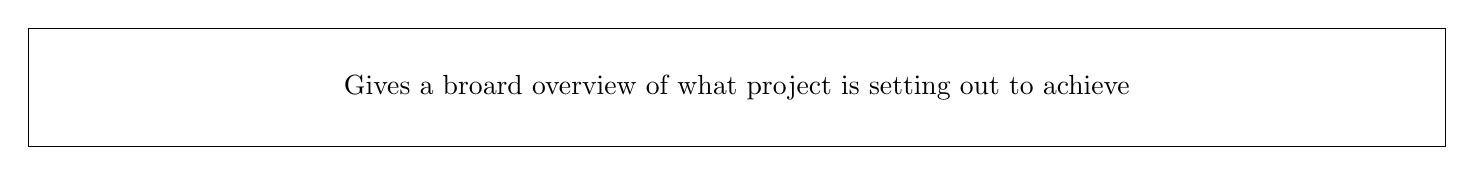
\begin{tikzpicture}
\draw (0,0) rectangle (18,1.5) node[pos=.5] {Gives a broard overview of what project is setting out to achieve};
\end{tikzpicture}

\section{Project Deliverables}
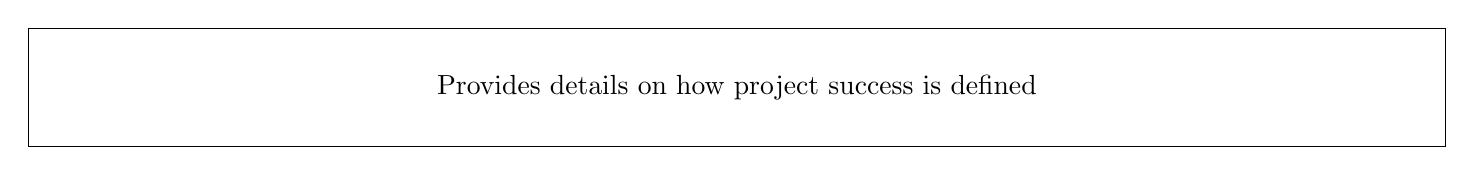
\begin{tikzpicture}
\draw (0,0) rectangle (18,1.5) node[pos=.5] {Provides details on how project success is defined};
\end{tikzpicture}

\section{Acceptance Criteria}
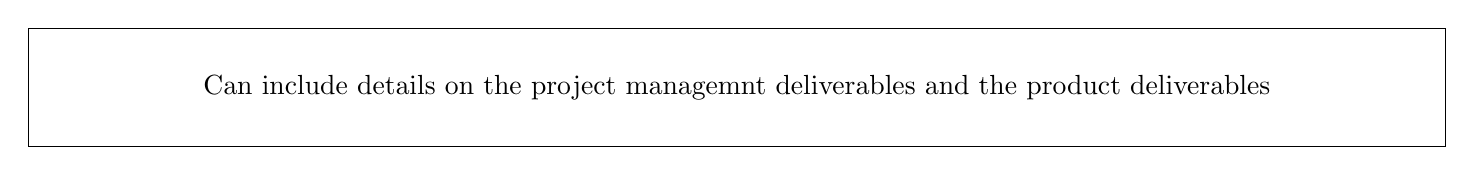
\begin{tikzpicture}
\draw (0,0) rectangle (18,1.5) node[pos=.5] {Can include details on the project managemnt deliverables and the product deliverables};
\end{tikzpicture}

\section{Constraints}
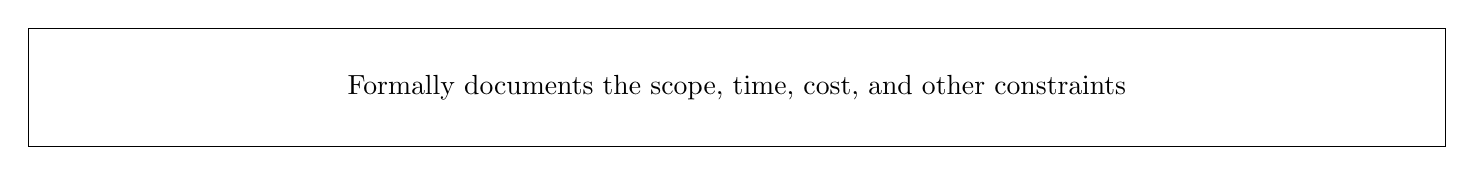
\begin{tikzpicture}
\draw (0,0) rectangle (18,1.5) node[pos=.5] {Formally documents the scope, time, cost, and other constraints};
\end{tikzpicture}

\section{Assumptions}
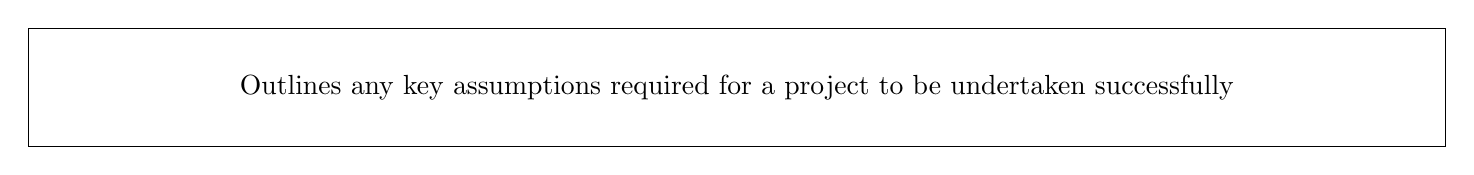
\begin{tikzpicture}
\draw (0,0) rectangle (18,1.5) node[pos=.5] {Outlines any key assumptions required for a project to be undertaken successfully};
\end{tikzpicture}

\end{document}